\section{Design and implementation}

\begin{figure}[t]   %% START_FIGURE
\centerline{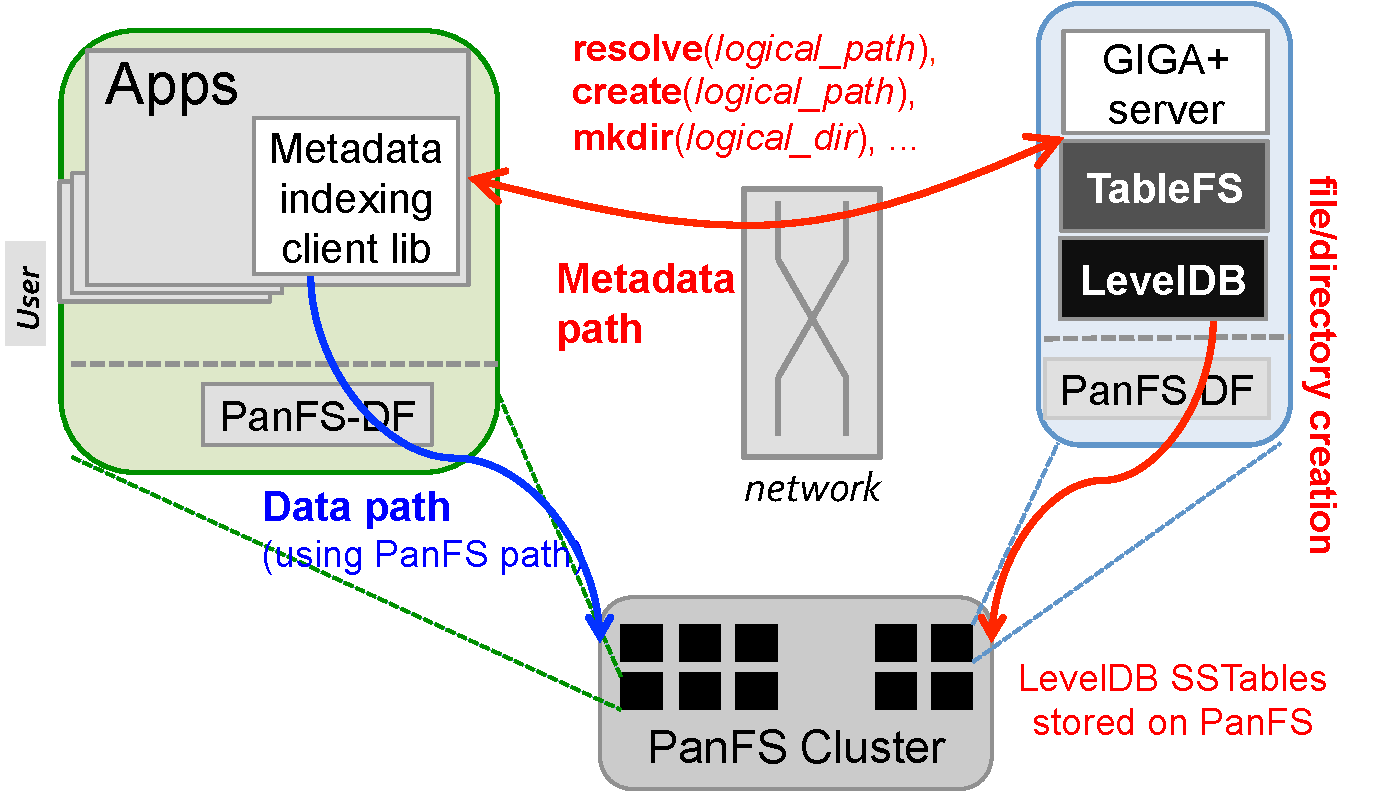
\includegraphics[scale=0.4]{./figs/giga-impl-leveldb-clusterfs}}
\vspace{10pt}
\caption{\textit{\footnotesize
Our scalable metadata service integrates two components: GIGA+ \cite{GIGA11},
a highly parallel and load-balanced indexing technique 
to partition metadata over multiple servers, and TableFS \cite{TableFS},
an optimized on-disk metadata representation on each server.
This integrated solution is layered on top of an existing cluster
file system deployment (PanFS) to improve metadata
and small file operation efficiency.
}}
%\vspace{10pt}
\hrule
\label{fig:design}
\end{figure}       %% END_FIGURE

Figure \ref{fig:design} presents the overall architecture of our scalable
metadata service. Our metadata service is a middleware inserted into
existing deployments of cluster file systems to improve metadata efficiency
while maintaining high I/O bandwidth for data transfers.
The system uses a client-server architecture,
and consists of three core components:

\begin{itemize}
\item{\textbf{Client:}} Applications interact with our middleware
through FUSE user-level file system \cite{fuse},
through a library linked into the application
or through a module in a common library such as MPI-IO.
The stateless client-side code redirects applications' file operations
to appropriate destinations according to the types of operations.
All metadata requests (e.g. \texttt{create()} and \texttt{mkdir()}),
and data requests to small files (e.g. \texttt{read()} and \texttt{write()}),
are handled through the metadata indexing modules that address
requests to the appropriate metadata indexing server.
For all data operations to large size files, the client code forwards
them directly to the underlying cluster file system to take full
advantage of data I/O bandwidth.

\item{\textbf{Metadata Indexing Server:}}
Each indexing server manages its local metadata storage backend to store and
access all metadata information and small file data. It uses GIGA+ algorithm to
partition large directory across indexing servers. It also monitors the growth
of small files, and migrates files into the underlying cluster file system
when their sizes exceed the threshold.

\item{\textbf{Metadata Storage Backend:}}
Metadata storage backend is a modified version of \tfs which packs metadata and
small file data into flat files, and stores flat files
in the underlying cluster file system. Since \tfs converts random updates into
sequential writes, it greatly improves metadata performance. In order to
dynamically distribute large directories, metadata storage backend also modifies
\tfs to support exporting and importing flat files in a batch.

\end{itemize}


Using \giga and \tfs enables us to tackle two key challenges: highly
concurrent metadata distribution for ingest-intensive parallel applications
such as check-pointing \cite{PLFS} and
optimized metadata representation that stores all file system
metadata in structured, indexed files managed by existing cluster file system
deployments.

Remainder of this section describes more details of our system.
Section \ref{design.giga} presents a primer on how \giga distributes metadata.
Section \ref{design.tablefs} shows how \tfs stores all file system metadata
and small files using a single on-disk structure on each server.
Section \ref{design.integration} focus on the challenges in effectively
integrating \giga and \tfs to work with existing cluster file systems.


\subsection{Distributed Metadata Indexing}
\label{design.giga}
\giga is a distributed hash-based indexing technique that incrementally
divides each directory into multiple partitions that are spread over multiple
servers \cite{GIGA11}.
Each filename stored in a directory entry is hashed and mapped to a partition
using an index.
\giga selects a hash partition such that for any distribution of unique filenames, the hash values of 
these filenames will be uniformly distributed in the hash space.
In addition to load-balanced distribution, \giga also grows the directory
index incrementally, i.e. all directories start small on a single server, and
then expand to more servers as they grow in size.

The core idea behind \giga is parallel splitting: each server splits
without system-wide serialization or synchronization.
Every server makes a local decision, without coordinating with other servers,
about when to split a partition.
Such uncoordinated growth causes \giga servers to have a partial view of the
entire index; there is no central server that holds the global view of the
partition-to-server mapping.
Each server knows about the partition it stores and the
identity of another server that knows more about each ``child'' partition
resulting from a prior split by this server.
This information is known as the per-server split history of its partitions.
The full \giga index is a transitive closure of the split history on each
server and represents the lineage of directory partitioning.

The full index (and split history) is also not maintained synchronously by any client.
\giga clients can enumerate the partitions of a directory by traversing
its split histories starting with the first partition that was created during
\texttt{mkdir}.
However, such a full index that is cached by a client may be stale at
any time, particularly for rapidly mutating directories.
\giga allows clients to keep using the stale mapping information and
receiving mapping updates from servers.
More discussion on the cost-benefit of using
inconsistent mapping state is not relevant to this work and can be found in
prior \giga{} literature \cite{GIGA07, GIGA11}.


\subsection{Metadata Storage Backend}
\label{design.tablefs}
Our metadata storage backend implements a modified version of \tfs
to manage all the metadata and small files on disk.
\tfs \cite{TableFS} is a stacked file system which uses another file system
as an object store, and organizes all metadata and small files in to a single
on-disk table using a Log-Structured Merge (LSM) tree \cite{ONeil1996}.
The reason for using LSM tree is that it buffers new and changed entries in
memory and translate small random disk writes into large sequential writes.
Therefore LSM tree can reduce random disk seeks effectively, and is a natural
fit for metadata intensive workloads. We decribe the structure of LSM tree
and how LSM tree is used in \tfs to store metadata in greater detail
in the following sections.

%\begin{figure}[!ht]
\begin{figure}[t]
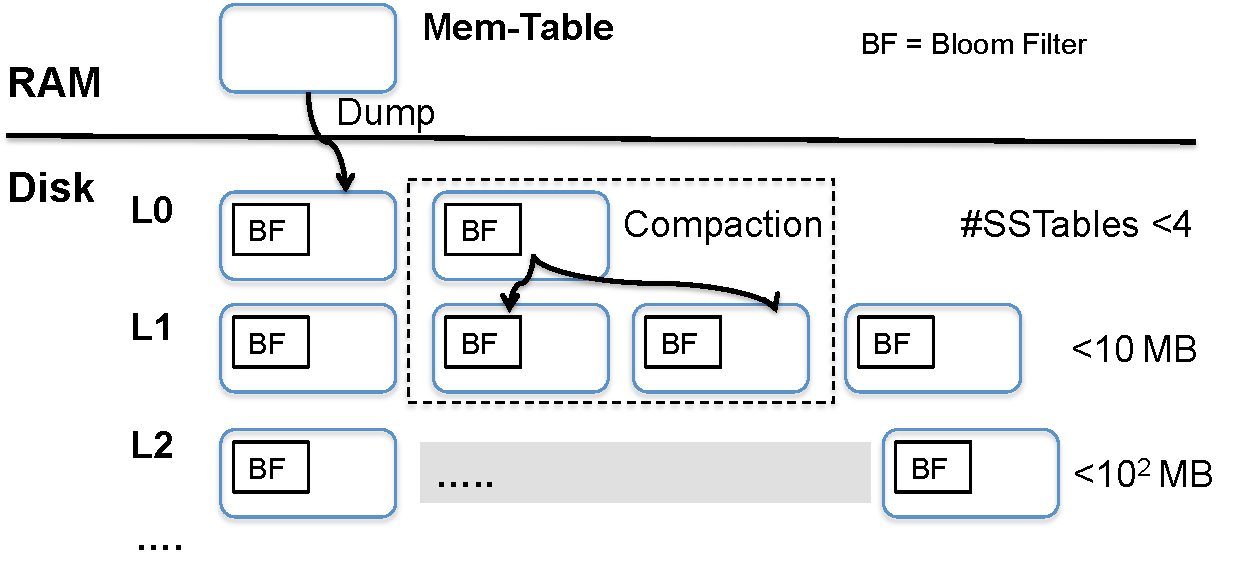
\includegraphics[scale=0.4]{figs/leveldb}
\vspace{10pt}
\caption{\textit{\footnotesize
LevelDB is an on-disk LSM-tree implementation that represents data in multiple 
files (called SSTables) containing sorted key-value pairs.
SSTables are grouped into different levels with lower-numbered levels
containing more recently inserted key-value pairs.
Finding a specific pair on disk may search up to all SSTables in level-0
and at most one in each higher-numbered level.
Compaction is the process of combining SSTables
by merge sort and moving combined SSTables into higher-numbered levels.
}}
%\vspace{10pt}
\hrule
\label{fig:leveldb}
\end{figure}


\textbf{LSM tree and LevelDB --}
\tfs uses an open-source implementation of LSM tree called LevelDB
\cite{LevelDB}. LevelDB provides a simple key-value store interface,
supporting point query and range query. In LevelDB, by default,
a set of changes are spilled to disk when the total size of modified
entries exceeds 4 MB.  When a spill is triggered, called a
minor compaction, the changed entries are sorted, indexed and written to disk
in a format called an SSTable \cite{BigTable}.  These entries may then be
discarded by the in memory buffer and can be reloaded by searching each SSTable
on disk, possibly stopping when the first match occurs if the SSTables are
searched most recent to oldest.  The number of SSTables that need to be
searched is reduced by maintaining a Bloom filter\cite{bloomfilter} on each,
but, with time, the cost of finding a record not in memory still increases.
Major compaction, or simply ``compaction",
is the process of combining multiple SSTables
into a smaller number of SSTables by merge sort.

As illustrated in Figure \ref{fig:leveldb},
LevelDB extends this simple approach to further
reduce read costs by dividing SSTables into levels.
In 0-th level, each SSTable may contain entries with any key value,
based on what was in memory at the time of its spill.
The higher-numbered levels of LevelDB's SSTables are
the results of compacting SSTables from their own or lower-numbered levels.
In levels excepth the 0-th level, LevelDB maintains the following invariant:
the key range spanning each SSTable is disjoint from
the key range of all other SSTables at that level.
So querying for an entry in the higher levels
only needs to read at most one SSTable in each level.
LevelDB also sizes each of the higher levels differentially:
all SSTables have the same maximum size and
the sum of the sizes of all SSTables at level $L$ will not exceed $10^L$ MB.
This ensures that the number of level grows
logarithmically with increasing numbers of entries.

~\\
\textbf{Table schema -- }
\tfs aggregates directory entries,
inode attributes and small files into one LSM tree
with an entry for each file and directory.
To translate the hierarchical structure of file system namespace
into key-value pairs, the 224-bit key is chosen to consist of
the 64-bit inode number of a entry's parent directory
and a 160-bit SHA-1 hash value of its filename string
(final component of its pathname).
The value of an entry contains the file's full name and inode attributes,
such as inode number, ownership, access mode, file size, timestamps (\textit{struct stat} in Linux).
For small files with size less than $T$, the value field also contains the file's data.
For large files, its file data is replaced by a symbolic link
that points to the actual file object in the underlying cluster file system.

%\begin{figure}[!ht]
\begin{figure}[t]
\centering
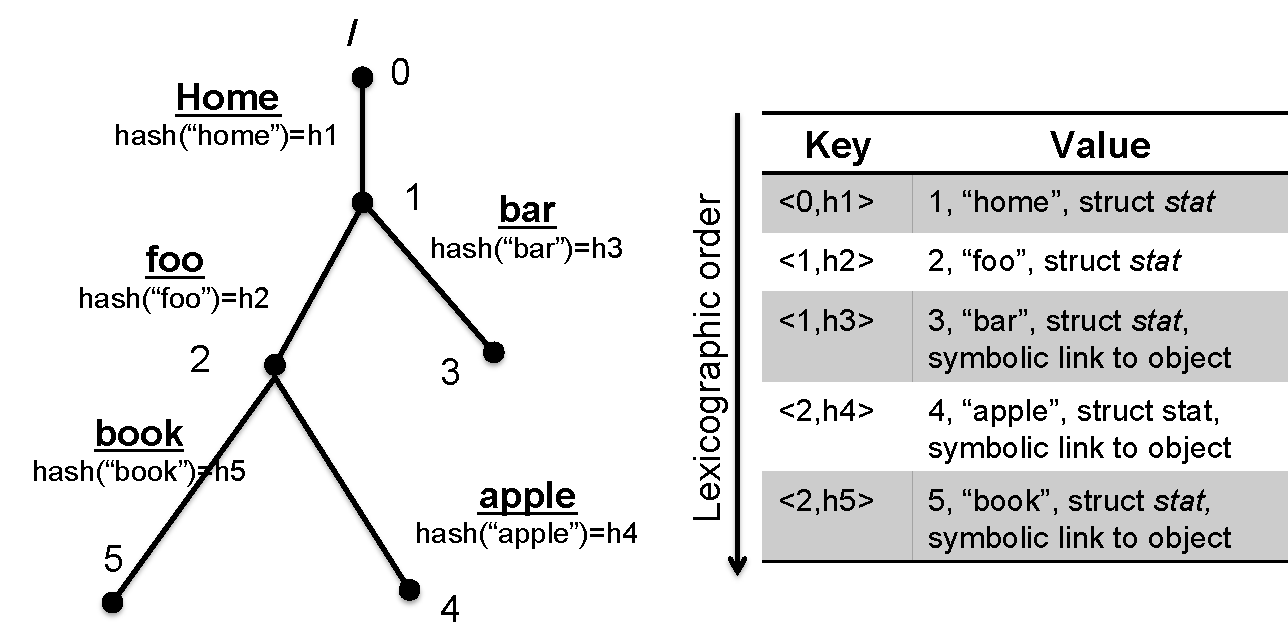
\includegraphics[scale=0.4]{figs/schema}
\vspace{10pt}
\caption{\textit{\footnotesize
An example illustrating a table schema for \tfs
to store metadata and file data as key-value pairs.}}
%\vspace{10pt}
\hrule
\label{fig:schema}
\end{figure}

Figure \ref{fig:schema} shows an example of representing
a sample file system's metadata into one table.
Embedding the inode number of parent directory into the key
helps with resolving the pathname.
Traversing the user's directory tree
only involves constructing a search key by concatenating the inode
number of current directory with the hash of
next component name in the pathname.
Another benefit is that all the entries in the same directory have rows that
share the same first 64 bits in their the table's key.
For $readdir$ operations, once the inode number
of the target directory has been retrieved,
a scan sequentially lists all entries having
the directory's inode number as the first 64 bits of their table's key.

Previous evaluation \cite{TableFS} has shown using \tfs schema with \ldb backend
can greatly improve metadata performance of the local file system.
Figure \ref{graph:ldb-singlenode} is taken from the original \tfs paper,
which compares the instantaneous throughput of FUSE-based \tfs
with three Linux file systems: Ext4 \cite{Ext4}, XFS \cite{XFS}, and
Btrfs \cite{BTRFS}.
The workload is to create 100 million zero-length files in a single directory.
All systems perform well at the beginning of the test, but the file create
throughput drops gradually for all systems.
Btrfs suffers the most serious throughput drop, slowing down to 100 operations
per second.
\tfs, however, maintains a more steady performance
with an average speed of 2,200 operations per second respectively,
\textit{and is 10X faster than all other tested file systems.}

\begin{figure}[t]  %%%%%%%%%%%%%%%%%%%%%%%
\centerline{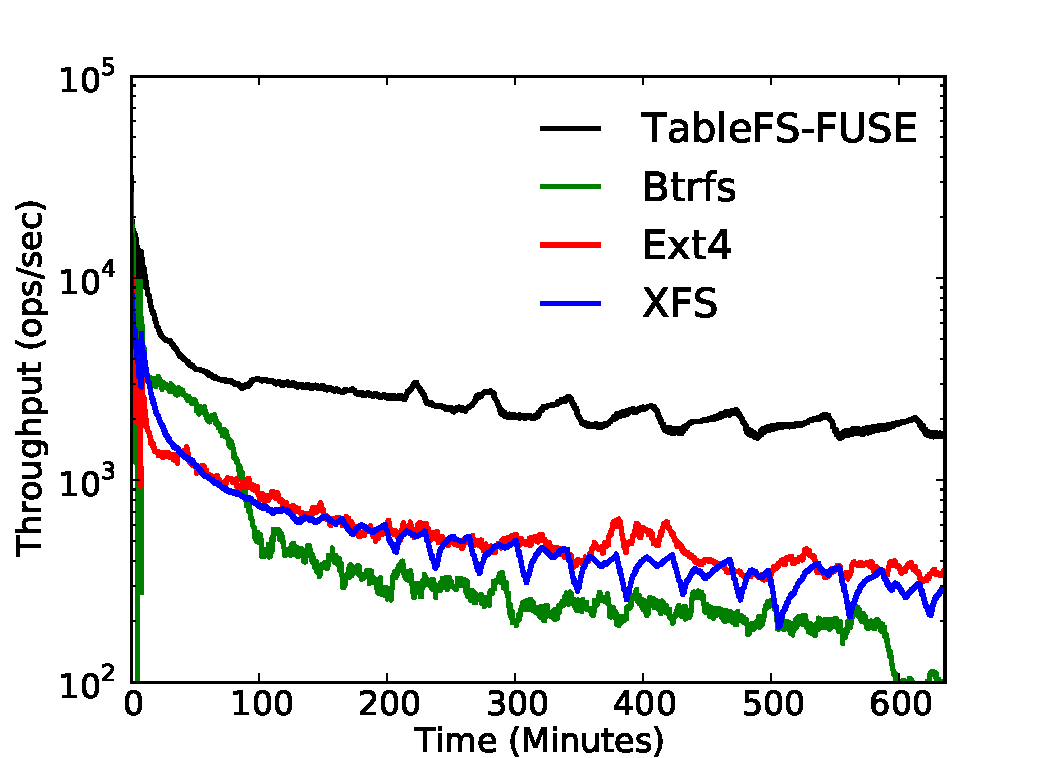
\includegraphics[scale=0.5]{./figs/ldb_insertrate_onenode}}
\vspace{10pt}
\caption{\textit{\footnotesize
This graph (from prior work \cite{TableFS}) shows
that the performance of single-node \tfs with FUSE is 10X faster than modern Linux
filesystems. The workload is to create 100 million zero-length files in one directory.
X-axis only shows the time until \tfs finished all insertions because the other
file systems were much slower. Y-axis has a logarithmic scale.}
}
%\vspace{10pt}
\hrule 
\label{graph:ldb-singlenode}
\end{figure}       %%%%%%%%%%%%%%%%%%%%%%%


\subsection{Integrating \giga{} and \tfs{}}
\label{design.integration}

To effectively build a middleware that integrates
the \giga distribution mechanism and \tfs,
we have to tackle two main challenges:
one is to modify \tfs to support for
migrating directory partition required by \giga;
the other is to decouple metadata and data paths to
achieve high performance for both paths.
This section discusses the modifications we made to
overcome the two challenges.


~\\
\textbf{Metadata representation -- }
\tfs stores all metadata including \giga hash
partitions for directories, entries in each hash partition, and other
bootstrapping information such as root entry and \giga configuration state.
The general schema used to store all file is:

\begin{table}[!htc]
\begin{tabular}{c|c}
key & \texttt{parentDirID,gigaPartitionID,hash(dirEntry)} \\
\midrule \\
value & \texttt{attr(dirEntry),[symlink|data|gigaMetaState]} \\
\end{tabular}
\label{tab:keyschema}
\end{table}

The main difference from the \tfs schema described in Section
\ref{design.tablefs} is the addition of two \giga specific fields:
\texttt{gigaPartitionID} to identify a
\giga hash partition and \texttt{gigaMetaState} to store the
hash partition related mapping information for directories.
These \giga related fields are used only
if large directories are distributed over multiple metadata servers.
A optimization is to eliminate \texttt{gigaPartitionID} in the key
by using the same hash function for both \giga and \tfs keys,
since the hash of entry name can determine the partition ID.

~\\
\textbf{Partition splitting -- }
The local \tfs instance stores \giga hash partitions and their directory
entries as SSTable Files in the underlying cluster file system.
Recall that each \giga server process splits a hash partition $P$ on
overflow and creates another hash partition $P'$ which is managed by a
different server; this split involves migrating approximately half the entries
from old partition $P$ to the new hash partition $P'$ on another server.
During splitting, the partition in migration has to be locked from
concurrent accessing for correctness.
We explored several ways to perform this cross-server partition split.

A straightforward solution would be to perform a range scan on
partition $P$, and remove about half the entries
(that will be migrated to the new partition $P'$) from $P$.
All removed entries are batched together
and sent in an RPC message to the server that will manage partition $P'$.
The split receiver inserts each key in the batch into its own \tfs instance.
While simplicity of this solution makes it attractive,
it is slow in practice and vulnerable to failures during splitting.
We have to devise a faster and safer technique to
reduce the time that the splitting range is locked.

The immutability of SSTables in \ldb makes such a fast bulk insert possible --
an SSTable can be added to Level 0 without its data being pushed through the
write-ahead log and minor compaction process.
To take advantage of this opportunity, we extended \tfs
to support a three-phase split operation:

\begin{itemize}
\item{Phase 1:} The split initiator performs a range scan on its \tfs instance
to find all entries in the hash-range that needs to be moved to another server.
Instead of packed into an RPC message,
the results of this scan are written in SSTable format to files in the
underlying cluster file system.

\item{Phase 2:} The split initiator notifies the split receiver about
the paths to the SSTable-format files in a much smaller RPC message.
Since these files are stored in shared storage,
the split receiver directly inserts these files as symbolic links
into the \ldb tree structure without actually copying these files.

\item{Phase 3:} The final step is a clean-up and commit phase:
after the receiver completes the bulk insert operation, it notifies the
initiator, who then deletes the migrated hash-range from its \tfs instance
and unlocks the range.
\end{itemize}

The three phases of splitting can be refined even further:
Assume that the splitting is initiated at the time $T_{split}$.
The split initiator can generate SSTables containing entries
older than $T_{split}$ without locking the hash range.
When the generation of SSTables with entries older than $T_{split}$ is finished,
the split initiator can lock the hash range and then write SSTables with
newly added or updated entries later than $T_{split}$.
By doing so, the duration of locking splitting hash range can be further reduced.
However, due to the code complexity of this optimization,
we left this optimization for future work.

~\\
\textbf{Decoupled data and metadata path -- }
All metadata and small file operations go through the \giga server;
however, following the same path for data operations on large files
would incur an unnecessary performance penalty of shipping data
over the network an extra time.
This penalty can be significant in HPC use-cases
where large files can easily be gigabytes to terabytes in size.

To avoid this penalty our middleware is designed to perform all
data-path operations of large files directly
through the cluster file system module in client machine.
Figure \ref{fig:design} illustrates this data path (in BLUE color).
Once the application tries to open a file with size greater than $T$,
our client library code will get back a symbolic link to the physical
path in the cluster file system, and open it locally.
All subsequent accesses to this large file will force
the client operating system to read/write through the native cluster file system client.
Thus applications can achieve the same data bandwidth.
FUSE-based clients can use the same trick but with additional overhead
of double context switching and memory copying \cite{PLFS}.
Recent work \cite{fuseopt} shows that FUSE kernel module can be modified
to make performance degradation less than $3\%$. We have not implemented
this modification in our current prototype.

While the file is open, some of its attributes (e.g., file size and last access time)
may change relative to \tfs's per-open copy of the attributes.
\giga servers monitor what large files are currently opened for access.
For attribute quires to these open files, \giga will directly query the underlying
cluster file system to get the most updated attributes.
Later \giga will synchronize these changes on file close on the metadata path.
Other attribute changes relative to permissions can be updated in-flight
through \giga servers.
By doing so, \giga servers can achieve the same level of metadata consistency
as provided by the underlying cluster file system.


\textbf{Layering on Panasas file system -- }
In PanFS \cite{PanFS}, \textit{Volume} is the basic logical unit
for administrators to manage the storage pool of PanFS.
The volume is a directory hierarchy with quota limit, and appears
as a directory below the single mount point of the whole storage system.
Each volume is only managed by a single metadata manager, but
the data of files created in the volume are spread over the entire storage pool.

A typical PanFS storage cluster may have multiple shelves,
each shelf consisting of one or two metadata managers and 9 or 10 storage nodes.
However, since a volume is assigned to a particular metadata manager,
all the metadata accesses to any files/directories in a volume
can only be served by that single metadata manager.

To take advantage of multiple metadata managers in PanFS,
our middleware load balance the storage of SSTables and large files across volumes.
Assume the case that we run the same number of \sys server processes
as the available metadata managers in PanFS.
\sys server processes can be run in the same machines that run PanFS metadata managers,
or in other machines behaving like proxies.
For each metadata manager, we create a volume and assign the volume
to a unique \sys server process.
The \sys server process then stores all the SSTables,
and large files in its managed directory partitions to it assigned volume.

\textbf{Fault tolerance -- }
The middleware design and techniques used for scaling the performance
of \sys does not impose any new major challenges on handling failures.
The primary functions required for fault tolerance include
replication of the \sys server's write-ahead logging for file system
state changes, detection of server failure, switching of backup servers,
and replaying of the replicated write-ahead log.
The replication of the write-ahead log may be not even necessary
if \sys is layered on a full-featured file system such as PanFS,
and the log can be replicated by the underlying file system.

For directory partition splitting and other operations requiring
distributed transactions (e.g.\texttt{ hardlink} and \texttt{rename}),
they can be implemented as a three-phase operation with protection
from write-ahead logging and garbaging collection of interrupted states.
\ldb also implements write-ahead logging and atomic batching operation
which can be used as primitives for fault tolerance in \tfs level.


The library version of client does not bring any new failure properties, either.
Directory-specific client state recovery is naturally supported by GIGA+
protocal, which only requires re-fetching the current server list and
rebuilding directory indexing by contacting speicfic servers.
For most operations except \texttt{open} and \texttt{close},
\sys server does not need to keep states for the clients.
Revoking the \texttt{open} handler for a large file can be achieved by
maintaining lease in the server side,
or by polling states from the underlying file system that
supports such functionality (e.g. PanFS).
The migration of small files from \tfs to the underlying file system is
handled by the \sys server, and is protected by the write-ahead logging.
